\section{Gauss-Jordan Elimination}
\label{sec:gauss-jordan-elimination}

Probably the most well-known algorithm for solving a
\hyperref[def:linear-system]{linear system} is the \emph{Gauss-Jordan
elimination}. As its name partially implies, its heart lies in the successive
\emph{elimination} of variables until only a single linear equation in one
variable stands unsolved. This is done by applying different
\emph{transformations} to the initial system that are guaranteed not to alter
the solution. We're going to solve a linear system first and describe the
general method second.

\begin{problem}{}{gauss-jordan-elimination}
 Solve the linear system
 \[
  \begin{array}{rcrcrcr}
   & & & & 3x_3 & = & 9\\
   x_1 & + & 5x_2 & - & 2x_3 & = & 2\\
   \frac{1}{3}x_1 & + & 2x_2 & & & = & 3
  \end{array}.
 \]
\end{problem}
\begin{probsol}
 We aim to transform the system step by step to a form which allows us to
 (successively) eliminate all variables.

 The first transformation entails a simple exchange of the first and third row.
 \begin{center}
  \begin{tikzpicture}
   \node (eq) at (0,0) {$
     \begin{array}{rcrcrcr}
      \frac{1}{3}x_1 & + & 2x_2 & & & = & 3\\
      x_1 & + & 5x_2 & - & 2x_3 & = & 2\\
      & & & & 3x_3 & = & 9
     \end{array}
   $};
  \coordinate (eqsw) at ($(eq.south west) + (-0.2,0.36)$);
  \coordinate (eqnw) at ($(eq.north west) - (0.2,0.36)$);
  \draw[<->,thick] (eqsw) to[bend left=90,looseness=2] (eqnw);
  \node at (-4.9,0) {\footnotesize \texttt{Swapped first and third row.}};
  \end{tikzpicture}
 \end{center}
 Next, we scale the first row by a factor of $3$.
 \begin{center}
  \begin{tikzpicture}
   \node (eq) at (0,0) {$
     \begin{array}{rcrcrcr}
      x_1 & + & 6x_2 & & & = & 9\\
      x_1 & + & 5x_2 & - & 2x_3 & = & 2\\
      & & & & 3x_3 & = & 9
     \end{array}
   $};
  \coordinate (eqnw) at ($(eq.north west) - (0.2,0.36)$);
  \coordinate (start) at ($(eqnw) - (1,0)$);
  \draw[->,thick] (start) to node[midway,yshift=2mm] {\footnotesize
   $\mathtt{\cdot 3}$} (eqnw);
  \node at ($(start) - (2,0)$) {\footnotesize \texttt{Scaled the first row by
   3.}};
  \end{tikzpicture}
 \end{center}
 Finally, we subtract the first row from the second row. Said in a more
 foreshadowing manner, we add the $(-1)$-multiple of the first row to the second
 row.
 \begin{center}
  \begin{tikzpicture}
   \node (eq) at (0,0) {$
     \begin{array}{rcrcrcr}
      x_1 & + & 6x_2 & & & = & 9\\
       & - & x_2 & - & 2x_3 & = & -7\\
      & & & & 3x_3 & = & 9
     \end{array}
   $};
  \coordinate (row1) at ($(eq.north west) - (0.2,0.36)$);
  \coordinate (row2) at ($(eq.west) - (0.2,0)$);
  \draw[->,thick] (row1) to[bend right=90,looseness=2] node[midway,xshift=-4mm]
   (mid) {\footnotesize $\mathtt{\cdot (-1)}$} (row2);
  \node at ($(mid) - (3.5,0)$) {\footnotesize \texttt{Subtracted the first row
   from the second.}};
  \end{tikzpicture}
 \end{center}
 These transformations have wrought the system into a state where it can be
 easily solved.

 Indeed, we immediately see that the third equation implies $x_3 = 3$.
 Substituting into the second equation gives 
 \[
  -x_2 - 2 \cdot 3 = -7
 \]
 whose solution is $x_2 = 1$. Finally, knowing the value of $x_2$, we can solve
 the first equation by another substitution. We get
 \[
  x_1 + 6 \cdot 1 = 9,
 \]
 thus $x_1 = 3$ and the triple $(3,1,3)$ is the \emph{unique} solution of the
 system.
\end{probsol}

Observant readers might have already identified the `kinds' of transformations
that were used in solving the \hyperref[prob:gauss-jordan-elimination]{linear
system above}. Nonetheless, we're about to spell them out.

The transformations that do not change the solution of a
\hyperref[def:linear-system]{linear system} include
\begin{enumerate}
 \item swapping two equations;
 \item scaling an equation by a non-zero constant;
 \item adding a multiple of an equation to \emph{another} equation.
\end{enumerate}
Note that transformations (2) and (3) come with sensible restrictions. Scaling
an equation by $0$ clearly changes the set of solutions of the system as it
basically removes the equation entirely. Adding a multiple of an equation to
\emph{itself} suffers from the same problem; it might result in `invalidating'
the equation should the scaling factor be $-1$.

We know proceed to prove that transformations (1) - (3) truly do not alter the
solutions of the initial system.

\begin{theorem}{Gauss-Jordan}{gauss-jordan}
 The transformations (1) - (3) of a linear system outlined above do not change
 its solution set.
\end{theorem}
\begin{thmproof}
 We will cover transformation (3) here. The proofs for transformations (1) and
 (2) are similar and thus left as an exercise.

 Consider the linear system
 \[
  \begin{array}{rcrcccrcr}
   a_{1,1}x_1 & + & a_{1,2}x_2 & + & \cdots & + & a_{1,n}x_n & = & c_1\\
   a_{2,1}x_1 & + & a_{2,2}x_2 & + & \cdots & + & a_{2,n}x_n & = & c_2\\
              &   &            &   &        &   &            & \vdots &\\
   a_{m,1}x_1 & + & a_{m,2}x_2 & + & \cdots & + & a_{m,n}x_n & = & c_m
  \end{array}
 \]
 of $m$ equations in variables $x_1,\ldots,x_n$ and let $(b_1,\ldots,b_n)$ be
 one of its solutions. Choose a constant $k$ and add the $k$-multiple of the
 $i$-th equation to the $j$-th equation for some indices $i \neq j \in
 \{1,\ldots,m\}$. Hence, the $j$-th equation of the system gets replaced by
 \[
  (a_{j,1} + k \cdot a_{i,1})x_1 + (a_{j,2} + k \cdot a_{i,2})x_2 + \cdots +
  (a_{j,n} + k \cdot a_{i,n})x_n = c_j + k \cdot c_i,
 \]
 which can be rearranged to
 \begin{equation}
  \label{eq:gauss-jordan}
  a_{j,1}x_1 + a_{j,2}x_2 + \cdots + a_{j,n}x_n + k \cdot (a_{i,1}x_1 +
  a_{i,2}x_2 + \cdots + a_{i,n}x_n) = c_j + k \cdot c_i.
 \end{equation}
 Since $(b_1,\ldots,b_n)$ is a solution of the original system, we know that
 \[
  \begin{array}{rcrcccrcr}
   a_{i,1}b_1 & + & a_{i,2}b_2 & + & \cdots & + & a_{i,n}b_n & = & c_i\\
   a_{j,1}b_1 & + & a_{j,2}b_2 & + & \cdots & + & a_{j,n}x_n & = & c_j
  \end{array}.
 \]
 Substituting this into equation~\eqref{eq:gauss-jordan} gives
 \[
  c_j + k \cdot c_i = c_j + k \cdot c_i,
 \]
 hence $(b_1,\ldots,b_n)$ is also the solution of the transformed system, as
 required.
\end{thmproof}

\begin{exercise}{}{gauss-jordan}
 Show that transformations (1) and (2) also don't change the set of solutions of
 the transformed linear system.
\end{exercise}

\begin{definition}{Elementary operations}{elementary-operations}
 The transformations (1) - (3) outlined above are called \emph{elementary
 operations} or \emph{row operations}.
\end{definition}

As we've seen in \myref{problem}{prob:gauss-jordan-elimination}, the application
of transformations (1) - (3) has its purpose in preparing the system for a final
back-substitution, where the values of all variables save the first in a row are
known beforehand. A system which is `ready' to be solved by back-substitution is
said to be in \emph{echelon form}.

\begin{definition}{Echelon form}{echelon-form}
 In each row of a \hyperref[def:linear-system]{linear system}, the first
 variable with a non-zero coefficient is called the row's \emph{leading
 variable}.

 A linear system is in \emph{echelon form} (or \emph{upper triangular form}) if
 the leading variable in each row is at least one column to the right of the
 leading variable in the row above and all rows filled with zeroes are at the
 bottom.
\end{definition}

\begin{example}{}{echelon-form}
 The system
 \[
  \begin{array}{rcrcrcr}
   x_1 & + & 6x_2 & & & = & 9\\
    & - & x_2 & - & 2x_3 & = & -7\\
   & & & & 3x_3 & = & 9
  \end{array}
 \]
 \textbf{is} in echelon form whereas
 \[
  \begin{array}{rcrcrcr}
   2x_1 & + & 3x_2 & - & x_3 & = & 9\\
    & & 3x_2 & - & 2x_3 & = & 2\\
    x_1 & & & - & x_3 & = & 0
  \end{array}
 \]
 is \textbf{not}.
\end{example}

For now, we shall employ intuition and a nibble of foresight to guide our
transformation of a \hyperref[def:linear-system]{linear system} into its
\hyperref[def:echelon-form]{echelon form}. Later, we intend to present a precise
algorithm (that computers also use) that achieves this.

\begin{example}{}{echelon-form-2}
 We're going to put the system
 \[
  \begin{array}{rcrcrcr}
    x_1 & + & x_2 & & & = & 0\\
    2x_1 & - & x_2 & + & 3x_3 & = & 3\\
    x_1 & - & 2x_2 & - & x_3 & = & 3
  \end{array}
 \]
 into echelon form and solve it using back-substitution. We'll label the rows of
 the system by Roman letters and denote transformations accordingly. For
 example, adding a $3$-multiple of row one to row three would be written
 symbolically as $\mathtt{3 \cdot I + III}$.

 First, we need to get rid of the variable $x_1$ in rows \texttt{II} and
 \texttt{III}. This can be done by subtracting adequate multiples of row
 \texttt{I}.
 \begin{center}
  \begin{tikzpicture}
   \node at (-6,0) {$
    \begin{array}{rcrcrcr}
      x_1 & + & x_2 & & & = & 0\\
      2x_1 & - & x_2 & + & 3x_3 & = & 3\\
      x_1 & - & 2x_2 & - & x_3 & = & 3
    \end{array}
    $};
   \node (eq) at (0,0) {$
    \begin{array}{rcrcrcr}
      x_1 & + & x_2 & & & = & 0\\
      & - & 3x_2 & + & 3x_3 & = & 3\\
      & - & 3x_2 & - & x_3 & = & 3
    \end{array}
   $};
  \draw[|->,thick,shorten <=5pt, shorten >=5pt] ($(eq.west) - (2.5,0)$) to
   node[midway,yshift=2mm] {\footnotesize $\mathtt{-2I + II}$}
   node[midway,yshift=-2mm] {\footnotesize $\mathtt{-I + III}$} (eq.west);
  \end{tikzpicture}
 \end{center}
 We continue by subtracting row \texttt{II} from row \texttt{III}.
 \begin{center}
  \begin{tikzpicture}
   \node at (-6,0) {$
    \begin{array}{rcrcrcr}
      x_1 & + & x_2 & & & = & 0\\
      & - & 3x_2 & + & 3x_3 & = & 3\\
      & - & 3x_2 & - & x_3 & = & 3
    \end{array}
    $};
   \node (eq) at (0,0) {$
    \begin{array}{rcrcrcr}
      x_1 & + & x_2 & & & = & 0\\
      & - & 3x_2 & + & 3x_3 & = & 3\\
      & & & - & 4x_3 & = & 0
    \end{array}
   $};
  \draw[|->,thick,shorten <=5pt, shorten >=5pt] ($(eq.west) - (2.5,0)$) to
   node[midway,yshift=2mm] {\footnotesize $\mathtt{-II + III}$} (eq.west);
  \end{tikzpicture}
 \end{center}
 The system is now in \hyperref[def:echelon-form]{echelon form}. The equation in
 row \texttt{III} forces $x_3 = 0$. Substitution into row \texttt{II}
 immediately gives $x_2 = -1$ and one final substitution into row \texttt{I}
 yields $x_1 = 1$.

 Hence, the solution of the system is the triple $(1, -1, 0)$.
\end{example}

\begin{exercise}{}{echelon-form}
 Using \emph{Gauss-Jordan elimination} solve the systems from
 examples~\ref{exam:static-equations} and~\ref{exam:chemical-reactions}.
\end{exercise}

All the systems we've studied so far have had the same number of equations as
variables. This of course need not be the case in general. Thankfully,
Gauss-Jordan elimination can \emph{always} be used to determine the solution set
of a \hyperref[def:linear-system]{linear system}. However, this set can also be
empty or infinite in cases where the number of variables doesn't match the
number of equations. The following examples illustrate this.

\begin{example}{}{overdetermined-system-1}
 This system has more equations than variables.
 \begin{equation}
  \label{eq:overdetermined-system}
  \begin{array}{rcrcr}
    x_1 & + & 3x_2 & = & 1\\
    2x_1 & + & x_2 & = & -3\\
    2x_1 & + & 2x_2 & = & -2
  \end{array}
 \end{equation}
 Before we put it into \hyperref[def:echelon-form]{echelon form} and solve it,
 let us ponder what the solution set may look like. Intuitively, a linear
 equation is basically a `restraint' or `condition' on the range of possible
 values the present variables may attain. If there are three equations
 restraining only two variables, then this restraint may be too harsh and lead
 to the system having no solution at all. The only case where solution
 \emph{does} exist involves one of the equations being \emph{redundant} --
 providing no additional condition. Algebraically, this happens if said equation
 is a \hyperref[def:linear-combination]{linear combination} of the other two.

 To draw a `real-life' simile, imagine the price of an apple being \$5/kg and
 that of bananas, \$1.5/kg. Saying that 3 kg of apples and 4 kg of bananas cost,
 say, \$30 is simply false because we can calculate (by the information ere
 provided) that this amount actually costs \$21. The third condition on the
 price of apples and bananas contradicted the previous two; just as a third
 equation in a \hyperref[def:linear-system]{linear system} in two variables can
 contradict the first two equations. We tend to call such systems
 \emph{overdetermined} and will in time dedicate a section to finding a `good'
 approximation of their solution.

 To solve the system~\eqref{eq:overdetermined-system}, we transform it into
 echelon form. First, we subtract twice the first row from the other two.
 \begin{center}
  \begin{tikzpicture}
   \node at (-5.5,0) {$
    \begin{array}{rcrcr}
      x_1 & + & 3x_2 & = & 1\\
      2x_1 & + & x_2 & = & -3\\
      2x_1 & + & 2x_2 & = & -2
    \end{array}
   $};
   \node (eq) at (0,0) {$
    \begin{array}{rcrcr}
      x_1 & + & 3x_2 & = & 1\\
      & & -5x_2 & = & -5\\
      & & -4x_2 & = & -4
    \end{array}
   $};
  \draw[|->,thick,shorten <=5pt, shorten >=5pt] ($(eq.west) - (2.5,0)$) to
   node[midway,yshift=2mm] {\footnotesize $\mathtt{-2I + II}$}
   node[midway,yshift=-2mm] {\footnotesize $\mathtt{-2I + III}$}(eq.west);
  \end{tikzpicture}
 \end{center}
 Finally, we add $(-4 / 5)$-times row \texttt{II} to row \texttt{III}.
 \begin{center}
  \begin{tikzpicture}
   \node at (-6,0) {$
    \begin{array}{rcrcr}
      x_1 & + & 3x_2 & = & 1\\
      & & -5x_2 & = & -5\\
      & & -4x_2 & = & -4
    \end{array}
   $};
   \node (eq) at (0,0) {$
    \begin{array}{rcrcr}
      x_1 & + & 3x_2 & = & 1\\
      & & -5x_2 & = & -5\\
      & & 0 & = & 0
    \end{array}
   $};
  \draw[|->,thick,shorten <=5pt, shorten >=5pt] ($(eq.west) - (3,0)$) to
   node[midway,yshift=2mm] {\footnotesize $\mathtt{-(4 / 5)II + III}$}
   (eq.west);
  \end{tikzpicture}
 \end{center}
 Clearly, the third equation is \emph{redundant} because it provides no
 condition binding the values of the variables. Back-substitution yields $x_2 =
 1$ and $x_1 = -2$. As we've claimed (but not yet proven), row \texttt{III} is
 indeed a linear combination of rows \texttt{I} and \texttt{II}. In this
 particular case, it holds that $\mathtt{(2 / 5)I + (4 / 5)II = III}$.
\end{example}

\begin{example}{}{overdetermined-system-2}
 Contrast this system with the system~\eqref{eq:overdetermined-system} from
 \myref{example}{exam:overdetermined-system-1}.
 \[
  \begin{array}{rcrcr}
    x_1 & + & 3x_2 & = & 1\\
    2x_1 & + & x_2 & = & -3\\
    2x_1 & + & 2x_2 & = & 0
  \end{array}
 \]
 In this case, the exact same row operations transform the system into
 \[
  \begin{array}{rcrcr}
    x_1 & + & 3x_2 & = & 1\\
    & & -5x_2 & = & -5\\
    & & 0 & = & 2
  \end{array},
 \]
 which clearly has no solution. This is a case of one equation of the system
 contradicting the other two.
\end{example}

Naturally, the ambitious, purposeful and \emph{overdetermined} systems have
their disinterested and vagrant sisters -- the \emph{underdetermined} systems.
We style such the systems that are short on the number of variables as compared
to the number of equations. As an example, consider the system
\begin{equation}
 \label{eq:underdetermined-system}
 \begin{array}{r c r c r c r}
  x_1 & + & x_2 & + & x_3 & = & 0\\
      &   & x_2 & + & x_3 & = & 0
 \end{array},
\end{equation}
which already \textbf{is} in \hyperref[def:echelon-form]{echelon form}. In spite
of that, the typical back-substitution method is (without needed alterations)
rendered unusable by the presence of two variables in the last row.

The system~\eqref{eq:underdetermined-system} is \emph{underdetermined} in the
sense that not enough equations are present to pinpoint a \textbf{unique}
solution. Quite the opposite, this system has infinitely many solutions that all
depend on as many parameters as many equations are missing to bind the values of
the variables completely -- in this case, \emph{one}.

In cases like these, one typically proceeds the following way: let one of the
variables (say, $x_3$) in the last equation be \emph{a parameter}. For the sake
of clarity, we shall rename $x_3$ to $t$ to highlight its updated social status.
The system thus looks like this.
\[
 \begin{array}{r c r c r c r}
  x_1 & + & x_2 & + & t & = & 0\\
      &   & x_2 & + & t & = & 0
 \end{array}
\]
Now, $t$ is no longer a variable so the system is no longer underdetermined. We
solve it briskly by setting $x_2 = -t$ and substituting this into the first
equation to obtain $x_1=0$. Therefore, the solution to the
system~\eqref{eq:underdetermined-system} is $(0,-t,t)$.

The dependence of the system's solution on a parameter naturally means that its
solution set is infinite. Any choice for the value of $t$ gives one particular
solution -- say $(0,-1,1)$ or $(0,0,0)$.

We close the section off with a few exercises. The next section is dedicated to
the geometric interpretation of linear systems.

\begin{exercise}{}{linear-system-1}
 Use Gauss-Jordan elimination to solve the following system.
 \[
  \begin{array}{r c r c r c r}
   x_1 & &  & - & x_3 & = & 0\\
   3x_1 & + & x_2 & & & = & 1\\
   -x_1 & + & x_2 & + & x_3 & = & 4
  \end{array}
 \]
\end{exercise}

\begin{exercise}{}{linear-system-2}
 Each of the following systems is in echelon form. Determine their number of
 solutions (without calculation).
 \begin{center}
  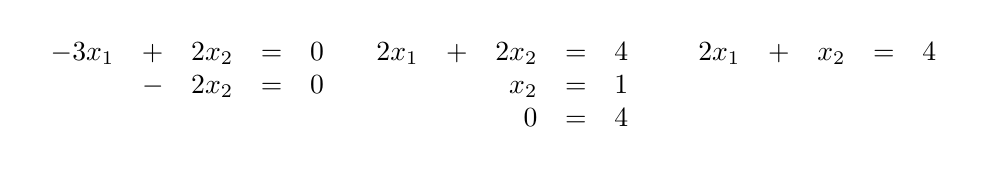
\begin{tikzpicture}
   \node at (0,0) {$
    \begin{array}{r c r c r}
     2x_1 & + & 2x_2 & = & 4\\
      & & x_2 & = & 1\\
       & & 0 & = & 4
    \end{array}
    $};
   \node at (-4,0) {$
    \begin{array}{r c r c r}
     -3x_1 & + & 2x_2 & = & 0\\
      & - & 2x_2 & = & 0\\
      & & & &
    \end{array}
    $};
   \node at (4,0) {$
    \begin{array}{r c r c r}
     2x_1 & + & x_2 & = & 4\\
      & & & &\\
      & & & &
    \end{array}
    $};
  \end{tikzpicture}
 \end{center}
\end{exercise}

\begin{exercise}{}{linear-system-3}
 Find the values of $a,b$ and $c$ that cause the graph of $f(x) = ax^2 + bx + c$
 to pass through the points $(1,2)$, $(-1,6)$ and $(2,3)$.
\end{exercise}

\begin{exercise}{}{linear-system-4}
 Show that for all numbers $a,b,c,d,j,k$ such that $ad - bc \neq 0$, the system
 \[
  \begin{array}{r c r c r}
   ax_1 & + & bx_2 & = & j\\
   cx_1 & + & dx_2 & = &k\\
    & & & &
  \end{array}
 \]
 has a \emph{unique} solution.
\end{exercise}
